\documentclass[12pt]{article}

% Language setting
% Replace `english' with e.g. `spanish' to change the document language
\usepackage[english]{babel}

% Set page size and margins
% Replace `letterpaper' with`a4paper' for UK/EU standard size
\usepackage[letterpaper,top=2cm,bottom=2cm,left=3cm,right=3cm,marginparwidth=1.75cm]{geometry}


%AMS-TeX packages
\usepackage{amssymb,amsmath,amsthm} 
\usepackage{geometry, graphicx}
\usepackage{tabulary}
\usepackage{physics}
\usepackage{enumitem}


% setup the margins
\geometry{margin=1.0in, headheight=15pt}

\usepackage[colorlinks=true, allcolors=blue]{hyperref}
%% Common Declarations %%


\title{PHSX 425, Exam 02}
\author{William Jardee}

\begin{document}
\maketitle

\section*{Question 1:}
\emph{An empty, hemispherical, stainless steel salad bowl of radius $R$ is electrically grounded at its point of contact with the table. The bowl spins with angular velocity $\omega$ about this point of contact, in a uniform vertical magnetic field of strength $B$. Find the elctrical potential at the rim of the bowl.}
\begin{figure}[h]
\centering
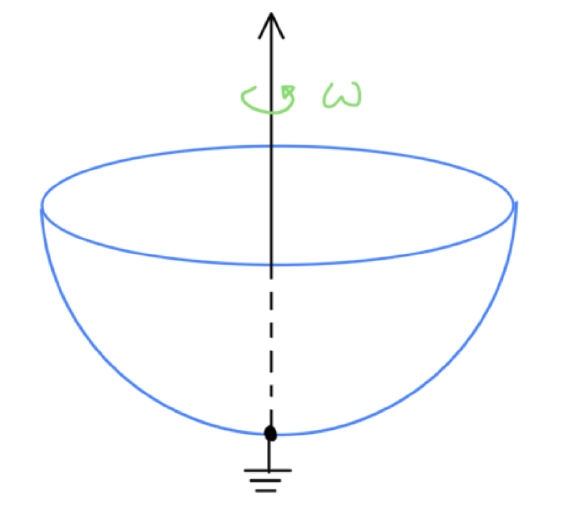
\includegraphics[scale=.5]{exam02_question1.png}
\label{fig:1.1}
\end{figure}

If we set up a cylindrical coordinate system such that $\hat{y}$ is parallel with $\vb{\omega}$, then we get the following set of parameters:
\[\vb{v} = \frac{\omega}{R}\hat{\theta} \qquad \vb{B} = B\hat{z}\]
Then, using the equation $\mathcal{E} = \oint (\vb{v} \times \vb{B})\cdot \dd{\vb{l}}$: $\vb{v} \times \vb{B} = \frac{\omega}{R} B \hat{s}$. Since the path that we are interested in is the rim of the bowl, then $\dd{\vb{l}}$ is in the $\hat{\theta}$ direction. 
\[\frac{\omega}{R} B \hat{s} \cdot \dd{l}\hat{\theta} = 0 \quad \rightarrow \quad \mathcal{E} = \oint (\vb{v} \times \vb{B})\cdot \dd{\vb{l}} = 0\]

I have a feeling that this one came out too easy and that I might have misunderstood that geometry of the problem. So, to add a little completion to the idea, I tried looking at all the surface that makes up the ``salad bowl". However, the same argument holds for every circle that you construct going down the side. 

And this kinda makes sense when I think of it. $\mathcal{E} = -\dv{\Phi}{t}$, and since our flux isn't changing at all, we should expect no introduction of potential. Another way to look at it is that the magnetic field doesn't do any work, so if it magically allowed for some potential to be created without any acceleration of the bowl it would be sketchy.  
\newpage

%---------------------------------------------------

\section*{Question 2:}
\emph{A toroidal coil with rectangular cross section has $n$ turns, with inner radius $a$ and outer radius $c$ as shown. It is wound on a form of non-magnetic material, $\mu = \mu_0$. At $s=b \, (a<b<c)$, an insulated wire is threaded between the windings of the coil, parallel to the $z$-axis. The rest of this wire is formed into a continuous loop, which closes outside the toroid. Find the mutual inductance between the wire loop and the coil.}
\begin{figure}[h]
\centering
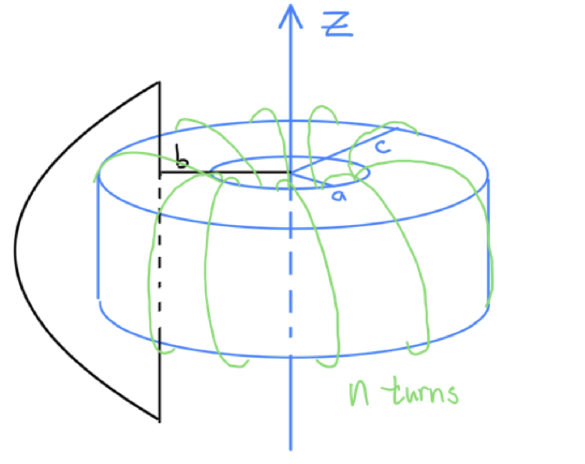
\includegraphics[scale=.5]{exam02_question2.png}
\label{fig:2.1}
\end{figure}

We have done this a hundred times, but I always forget; so, the first step is to calculate the B-field in the solenoid.
\[\oint \vb{H} \cdot \dd{\vb{l}} = I_\text{enc}\]
\[H\cdot 2 \pi s = In\]
\[\vb{H} = \frac{In}{2 \pi s} \hat{\phi}\]
Now, using $\vb{B} = \mu \vb{H}$ 
\[\vb{B} = \frac{\mu In}{2 \pi s} \hat{\phi}\]\bigskip

Now, we use use this to find the amount of the B-field from the toroid that actually passes through our funky loop.
\[h\int_b^c \frac{\mu I n}{2 \pi s} \dd{s}\]
\[=\frac{\mu h n I}{2 \pi}\ln\Big(\frac{c}{b}\Big)\]
\bigskip

Finally, we can use this to find the mutual inductance from the equation $\Phi_2 = M I_1$
\[IM = \Phi = \frac{\mu h n I}{2 \pi} \ln \Big(\frac{c}{b}\Big)\]
\[M = \frac{\mu n h}{2 \pi} \ln\Big(\frac{c}{b}\Big)\]

Quick sanity check to make sure that the jazz inside the natural log is unitless, and that the mutual inductance is only reliant on geometric values ... Great!

\newpage
%---------------------------------------------------

\section*{Question 3:}
\emph{A high-impedance voltmeter is connected to a wire of radius $a$ as shown. Assume that the current $I$ in the wire is uniformly distributed.}
\begin{figure}[h]
\centering
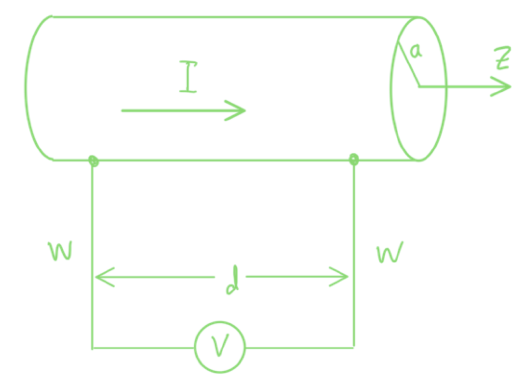
\includegraphics[scale=.5]{exam02_question3.png}
\label{fig:3.1}
\end{figure}

\begin{enumerate}[label=\alph*)]
\item \emph{If $I$ is constant, and the wire's resistivity is $k$, what voltage is measured?}\bigskip

The first step I took was to calculate the mutual inductance, that way I could check if there is any change in the voltage due to an EMF. 
\[\oint \vb{B}\cdot \dd{\vb{l}} = \mu_0 I_\text{enc}\]
\[B\cdot 2\pi s = \mu_0 I\]
\[B = \frac{\mu_0 I}{2 \pi s}\]\bigskip

\[\Phi = \int^{a+w}_a \frac{\mu_0 I}{2 \pi s} d \dd{s}\]
\[= \frac{\mu_0 I d}{2 \pi}\ln\Big(\frac{a+w}{a}\Big)\]
\[= \frac{\mu_0 I d}{2 \pi}\ln\Big(1+\frac{w}{a}\Big)\]\bigskip
\begin{equation}
M = \frac{\mu_0 d}{2 \pi}\ln\Big(1+\frac{w}{a}\Big)
\label{eq:3.1}
\end{equation}

Since $\mathcal{E} = \dv{\Phi}{t} = 0$, so the only voltage measured is from the Ohms Law.
\[\Delta V = \frac{I}{k \pi a^2}\]

\item \emph{Find the measure voltage $V(t)$ if the current is $I = I_0 e^{i\omega t}$. Assume that $w\omega \ll c$, where $c$ is the speed of light; why is this important?}\bigskip

We have two sources, both pointed out in the part a. Using $\mathcal{E} = \dv{\Phi}{t}$ and that value from \eqref{eq:3.1}:
\[\Delta V = \frac{I}{k \pi a^2} - \mathcal{E}\]
\[= \frac{I_0 e^{i\omega t}}{k \pi a^2}-\frac{\mu_0 d}{2 \pi} \ln\Big(1 + \frac{w}{a}\Big) I_0 i\omega e^{i \omega t} \]
\[\Delta V = \Big[\frac{1}{k \pi a^2}- i\omega \frac{\mu_0 d}{2 \pi} \ln\Big(1 + \frac{w}{a}\Big)\Big]I_0 e^{i \omega t} \]\bigskip

It is important that $w\omega \ll c$ because otherwise the speed that the electrons would have to near/overcome would be the speed of light. And, as we all know from our time with special relativity, lengths and time scales get weird when we near $\frac{1}{10} c$. Especially since we haven't dealt this this concept formally in class, we wouldn't know exactly how to deal with it.\footnote{It's an interesting thought, however. My first guess would be that there would be a battle between time dilation and length contraction going on. I'm not confident to say whether this idea is actually important, but, thinking about electrons skipping over atoms entirely in a pseudo runaway event. At this point we would be dealing with a plasma situation and I don't think simple wire setup like this is built to deal with that.} 

\end{enumerate}
\newpage

%---------------------------------------------------

\section*{Question 4:}
\emph{At $t=0$, an infinite conducting medium has free charge distribution $\rho_0(\textbf{r},0)$. The medium is also a linear dielectric, with dielectric constant $\varepsilon_r$, but $\mu = \mu_0$.}
\begin{enumerate}[label=\alph*)]
\item \emph{Find the free and bound charge densities as a function of time.}\bigskip

\par Let's first time the $\rho_b(\textbf{r},0)$, then I will provide an argument for how these two initial densities evolve with time. We know in a linear dielectric that
\[\rho_b = -\div{\vb{P}}= -\div{\varepsilon_0\frac{\chi_e}{\varepsilon}\vb{D}} = -\Big(\frac{\chi_e}{1+\chi_e}\Big)\rho_f = \frac{1-\varepsilon_r}{\varepsilon_r}\rho_f\]
\[\rho_b(\vb{r},0) = \frac{1-\varepsilon_r}{\varepsilon_r}\rho_f(\vb{r},0)\]
We already know that $\rho(\vb{r},t)=\rho(\vb{r},0)e^{-t/k\varepsilon_0}= (\rho_f(\vb{r},0)+\rho_b(\vb{r},0))e^{-t/k\varepsilon_0}$. At any point in time $\rho_{\text{tot}} = \rho_f+\rho_b$, so the free and bound densities must evolve in time in the same way that the total charge density, so we can just say:
\[\rho_f(\vb{r},t) = \rho_f(\vb{r},0)e^{-t/k\varepsilon_0}\]
\[\rho_b(\vb{r},t) = \frac{1-\varepsilon_r}{\varepsilon_r}\rho_f(\vb{r},0)e^{-t/k\varepsilon_0}\]

\item \emph{How are the free and polarization currents ($\textbf{J}_f, \textbf{J}_p$) related to the charge densities?}\bigskip

The first thing to note for this question is that $\mu = \mu_0(1+\chi_m) = \mu_0 \rightarrow \chi_m = 0$. So, $\vb{M} = 0$ and 
\[J_{\text{bound}} = \curl{\vb{M}} = 0\]
\[J = J_{\text{free}} + J_{\text{bound}} = J_{\text{free}}\]
So, since we know that $\dv*{\rho}{t} = -\div{J}$, 
\[-\div{\vb{J}} = \dv{t}\Big(\Big[\frac{1-\varepsilon_r}{\varepsilon_r} + 1\Big]\rho_f(\vb{r},0)e^{-t/k\varepsilon_0}\Big)\]
\[ = \Big[\frac{1}{\varepsilon_r}\Big]\rho_f(\vb{r},0)\Big(\frac{-\sigma}{\varepsilon_0}\Big)e^{-t/k\varepsilon_0}\]
\[ = \frac{-\sigma}{\varepsilon_0 \varepsilon_r}\rho_f(\vb{r},0)e^{-t/k\varepsilon_0}\]
So, altogether
\[\vb{J_\text{bound} = 0}\] 
\begin{equation}
\div{\vb{J}_\text{free}} = \frac{\sigma}{\varepsilon_0 \varepsilon_r}\rho_f(\vb{r},0)e^{-t/k\varepsilon_0}
\label{eq:4.b}
\end{equation}

\item \emph{Is there a resulting magnetic field?}\bigskip

\[\div{\vb{E}} = \frac{\rho}{\varepsilon_0}\]
\[\dv{t}\div{\vb{E}} = \dv{t}\frac{\rho}{\varepsilon_0}\]
This gives the same result as \eqref{eq:4.b}. So, when calculating $\curl{\vb{B}} = \mu_0\Big(\vb{J} + \varepsilon_0 \dv{\vb{E}}{t}\Big)$, we get 0. Since $\div{\vb{B}} = 0$ as well. So, put together:
\[\vb{B} = 0\]
 

\item \emph{Do your results agree with all four Maxwell's equations in matter, as given in Griffiths?}\bigskip

From Griffiths:
\begin{equation}
\div{\vb{D}} = \rho_f
\label{eq:max1}
\end{equation} 
\begin{equation}
\div{\vb{B}} = 0
\label{eq:max2}
\end{equation} 
\begin{equation}
\curl{\vb{E}} = -\pdv{\vb{B}}{t}
\label{eq:max3}
\end{equation} 
\begin{equation}
\curl{\vb{H}} = \mu_0\Big(\vb{J} + \varepsilon_0 \pdv{\vb{E}}{t}\Big)
\label{eq:max4}
\end{equation} 

To save being redundant, we used \eqref{eq:max1} to justify calculating $\rho_b$, so it must be consistent. We built $\vb{B}= 0 $ from combining \eqref{eq:max2} and \eqref{eq:max4},\footnote{when we realize that $\vb{M} = 0 \rightarrow \mu_0\vb{H} = \vb{B}$, then we get back to the equation that we used initially, which is one of the normal Maxwell's equations} so those are consistent. Finally, we can recognize that there is no source for a curl to $\vb{E}$, so it is good that is equal to zero and satisfy \eqref{eq:max3}.

\end{enumerate}

\end{document}